\chapter{Kravspecifikation}

\begin{figure}[htbp] \centering
\section{Aktører}
\fbox{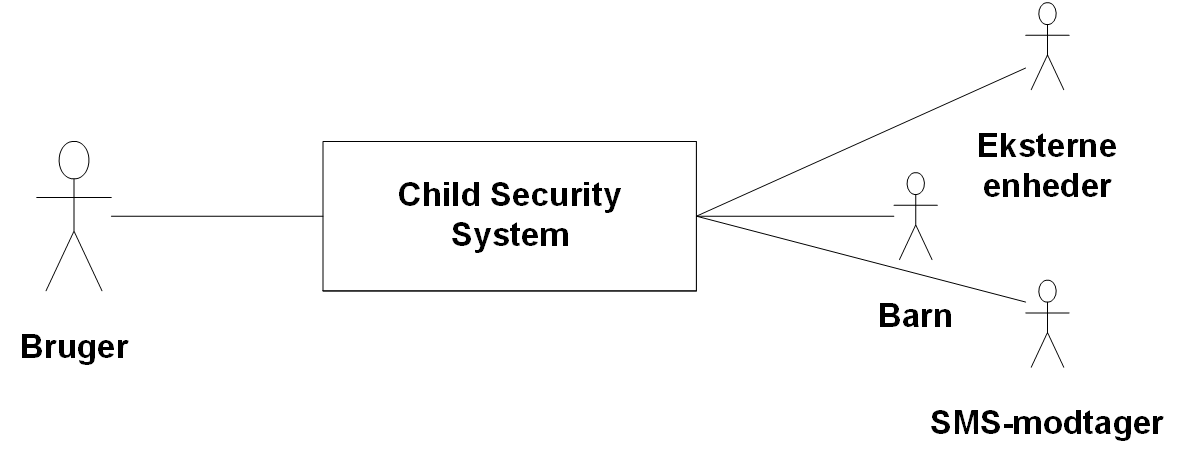
\includegraphics[width=\textwidth]{billeder/Kontekst_Diagram}}
\caption{Kontekst diagram}
\label{lab:kontekstdiagram}
\end{figure}

\begin{table}[!htbp] \centering
\subsection{Bruger}
\begin{tabular}{|p{4cm}|p{8cm}|}
	\hline
		\textbf{Type Beskrivelse} &
			Bruger aktøren er ejeren af systemet eller den voksne med adgang til Computeren. 
			Vil typisk være forældre, barnepige osv. (Primær) \\\hline
	\end{tabular}
\end{table}

\begin{table}[!htbp] \centering
\subsection{Eksterne enheder}
\begin{tabular}{|p{4cm}|p{8cm}|}
	\hline
		\textbf{Type Beskrivelse} &
			Eksterne enheder, omfatter hvad man ønsker at aflåse eller slukke for. 
			Vil typisk være skabe, komfur, el-kedel osv. (Sekundær) \\\hline
	\end{tabular}
\end{table}

\begin{table}[!htbp] \centering
\subsection{Barn}
\begin{tabular}{|p{4cm}|p{8cm}|}
	\hline
		\textbf{Type Beskrivelse} &
			Barnet eller børnene i huset, som systemet skal beskytte.	(Sekundær) \\\hline
	\end{tabular}
\end{table}

\begin{table}[!htbp] \centering
\subsection{SMS modtager}
\begin{tabular}{|p{4cm}|p{8cm}|}
	\hline
		\textbf{Type Beskrivelse} &
			Typisk forældrene eller barnepigen. Den person der skal have besked om gråd eller anden støj fra børneværelset. (Sekundær) \\\hline
	\end{tabular}
\end{table}

\begin{figure}[!htbp] \centering
\section{Usecases}
\vspace*{\fill}
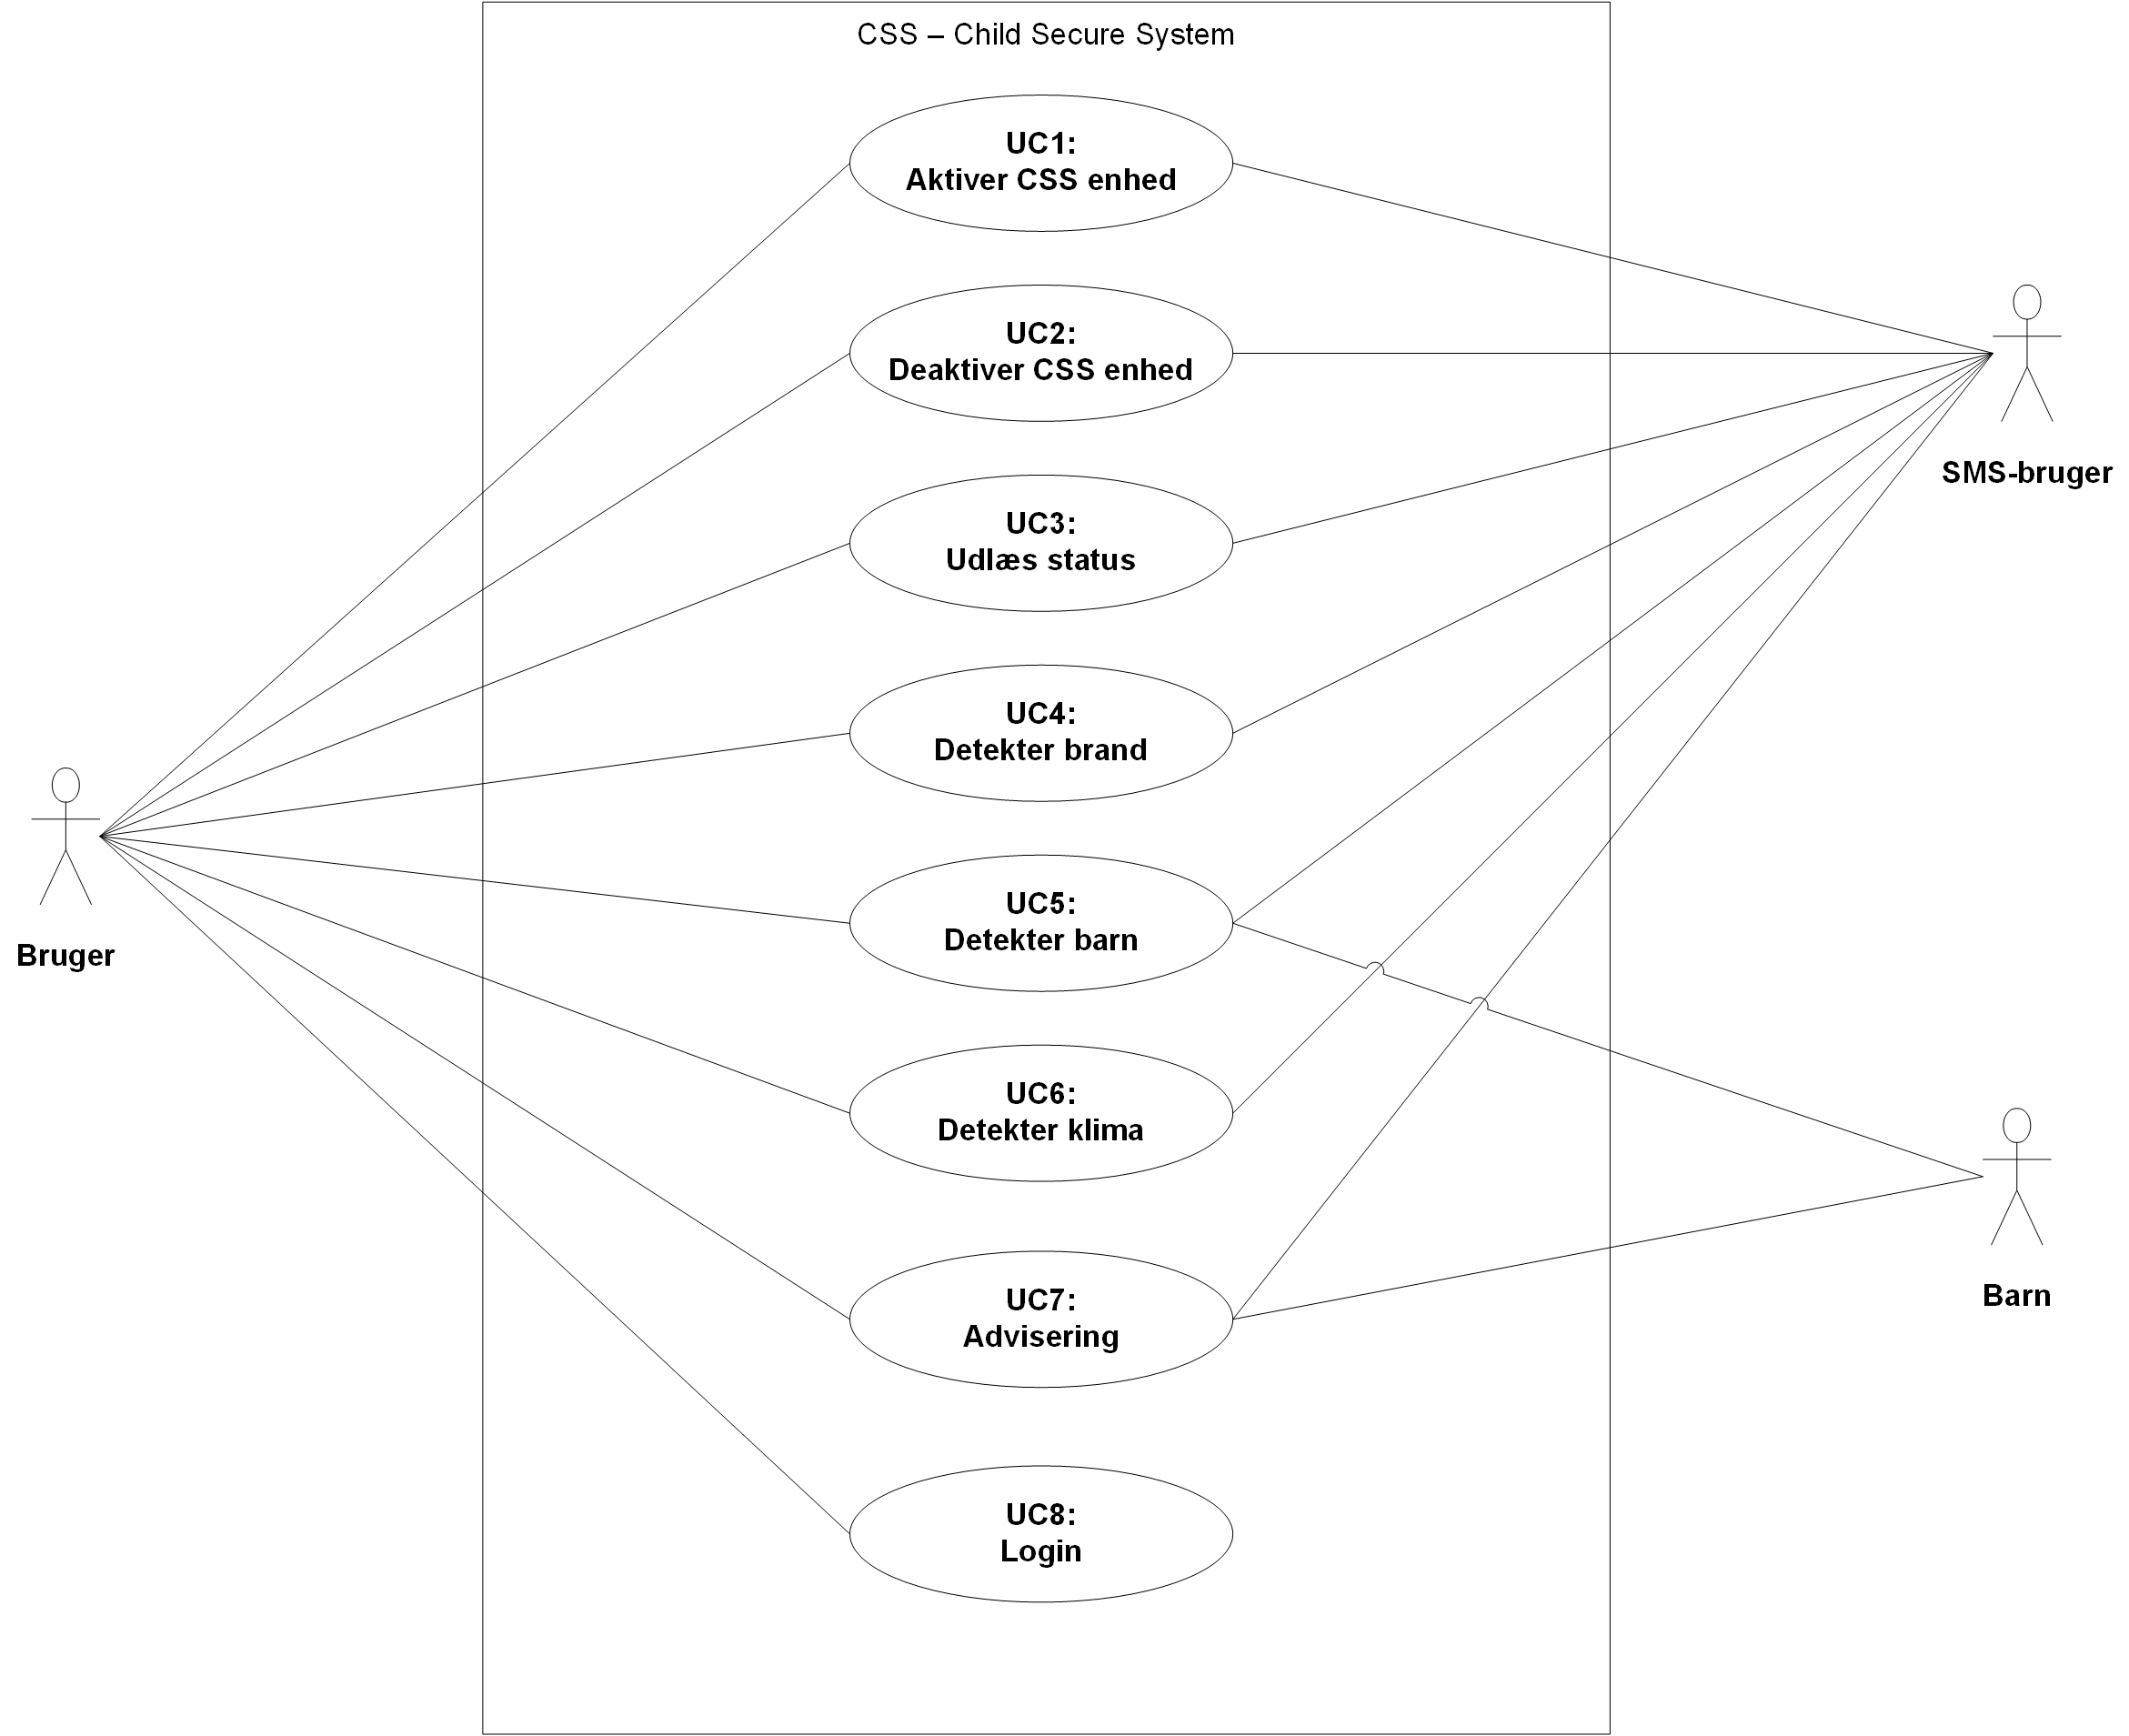
\includegraphics[width=\textwidth]{billeder/Usecase_Diagram}
\caption{Usecase diagram}
\label{lab:usecasediagram}
\vspace*{\fill}
\end{figure}

% UC1: Login

\subsection{UC1: Login}
\begin{center} \centering
	\begin{longtable}{|p{6cm}|p{8cm}|}
	\hline
		\multicolumn{2}{|l|}{\textbf{UC1: Login}} \\\hline
		\endfirsthead
		
		\multicolumn{2}{l}{...fortsat fra forrige side} \\ \hline 
		\multicolumn{2}{|l|}{\textbf{UC1: Login}} \\\hline
		\endhead		

\textbf{Mål}								
&At Bruger kan logge ind ved hjælp af adgangskode
 \\\hline
\textbf{Initialisering}					
&Bruger vælger login i interface
 \\\hline
\textbf{Aktører og Stakeholders}			
&Bruger(Primær), DE2 Board(Sekundær)
 \\\hline
\textbf{Referencer}						
&Ingen
 \\\hline
\textbf{Antal af samtidige hændelser}	
&1
 \\\hline
\textbf{Forudsætning}					
&At interfacet er tændt
 \\\hline
\textbf{Efterfølgende tilstand}			
&At bruger er logget ind og hovedmenu vises på skærmen. Hele systemet er klar til brug
 \\\hline
\textbf{Hovedforløb}						
& 
\begin{enumerate}

\item Bruger vælger login i interfacet

\item \label{UC2und1}Bruger indtaster 3 koder adskilt af ''Enter'' på DE2 board \newline
\textbf{[Undtagelse \ref{UC2und1}a]} Bruger vælger Annuller

\item Bruger får adgang til hovedmenuen	
 
\end{enumerate}
\\\hline

\textbf{Undtagelser}						
&\begin{enumerate}[label= \ref{UC2und1}a.]
			\item Bruger vælger annuller og kommer tilbage til loginskærm
		\end{enumerate}
\\\hline


		%\textbf{Version}		&1.0 \\\hline
	\end{longtable}
	\label{UC1} 
\end{center}

% UC2: Aktiver

\subsection{UC2: Aktiver}
\begin{table}[H] \centering
\begin{tabular}{|p{6cm}|p{8cm}|}
	\hline
\multicolumn{2}{|l|}{\textbf{UC2: Deaktiver CSS enhed(er)}} \\\hline
\textbf{Mål}	&
At brugeren kan deaktivere enkelte eller alle enheder, i systemet.
\\\hline
\textbf{Initialisering} &
Bruger trykker "deaktiver", og bliver
præsenteret for hvilke enheder der skal deaktiveres, samt en mulighed for at deaktivere alle
enheder. 
\\\hline
\textbf{Aktører og Stakeholders}	&
Bruger er hovedaktør
\\\hline
\textbf{Referencer} &
Login
\\\hline
\textbf{Antal af samtidige hændelser} &
1
\\\hline
\textbf{Forudsætning} &
At CSS Systemet er helt eller delvist aktiveret.
\\\hline
\textbf{Efterfølgende tilstand} &
Hovedmenu vises
\\\hline
\textbf{Hovedforløb}	&
Bruger trykker deaktiver og følger instruktionerne på skærmen.
\begin{enumerate}
\item Deaktiver alt
\item Deaktiver alle låse
\item Deaktiver babylarm
\end{enumerate}
\\\hline
\textbf{Undtagelser}	&
Ingen
\\\hline
\textbf{Version}		&1.0 \\\hline
	\end{tabular}
	\label{tab:UC2} 
\end{table}

% UC3: Deaktiver

\subsection{UC3: Deaktiver}
\begin{table}[H] \centering
	\label{tab:UC3}
\begin{tabular}{|p{6cm}|p{8cm}|}
	\hline
		\textbf{Mål}						&At Bruger kan deaktivere enkelte eller alle enheder, i systemet. \\\hline
		\textbf{Initialisering} 			&Bruger vælger ''Deaktiver'' \\ \hline
		\textbf{Aktører og Stakeholders}	&Bruger(Primær), Eksterne enheder(Sekundær)\\ \hline
		\textbf{Referencer} 				&UC1: Login \\ \hline
		\textbf{Antal af samtidige hændelser} &1 \\ \hline
		\textbf{Forudsætning} 			&Systemet er tændt \\ \hline
		\textbf{Efterfølgende tilstand} 	&Enkelte eller alle enheder er deaktiveret \\ \hline
		\textbf{Hovedforløb}				&

	\begin{enumerate}	
						
					
				\item Bruger vælger ''Deaktiver'' i hovedmenu (UC1 gennemføres)
										
				\item \label{uc3menu}UI viser mulige enheder samt ''Vælg alle'', ''Deaktiver''  og ''Tilbage''
												
				\item Bruger markerer ønskede enheder til deaktivering
												
				\item \label{uc3deact} Bruger vælger ''Deaktiver''\newline
					\textbf{[Undtagelse \ref{uc3deact}a]} Bruger vælger ''Tilbage''
												
				\item \label{uc3sysdeact} Systemet deaktiverer valgte enheder \newline
					\textbf{[Undtagelse \ref{uc3sysdeact}a]} Ingen valgte enheder
				
				\item UI viser besked om at enheder, er deaktiverede
																	
				\item UI returnerer til hovedmenu	
	
	\end{enumerate} \\ \hline

		\textbf{Undtagelser}	
		
		&\begin{enumerate}[label= \ref{uc3deact}a.]
			\item UI returnerer til hovedmenu og UC3 afbrydes
		\end{enumerate}						
							
		\begin{enumerate}[label= \ref{uc3sysdeact}a.]
			\item Hvis ingen enheder er valgt udskrives en fejl på skærmen og beder brugeren om at vælge en enhed og går til UC3.\ref{uc3menu}
		\end{enumerate} \\\hline
											
		%\textbf{Version}		&1.2 \\\hline
		
	\end{tabular} 
\end{table}

% UC4: Udlæs status

\subsection{UC4: Udlæs status}
\begin{table}[H] \centering
\begin{tabular}{|p{6cm}|p{8cm}|}
	\hline
\multicolumn{2}{|l|}{\textbf{UC4: Detekter brand}} \\\hline
\textbf{Mål}								&At detektere en opstået brand og eller røgudvikling \\\hline
\textbf{Initialisering}					& CO_2 \\\hline
\textbf{Aktører og Stakeholders}			&Primær: Bruger ønsker at få besked om brand \\\hline
\textbf{Referencer}						& Ingen \\\hline
\textbf{Antal af samtidige hændelser}	& 1 pr. sensor \\\hline
\textbf{Forudsætning}					& CSS sensor aktiv  \\\hline
\textbf{Efterfølgende tilstand}			& Besked til bruger - CSS sensor aktiv \\\hline
\textbf{Hovedforløb}						&  1. CSS sensor aktiv 2. CSS sensor detekterer CO_2  3. CSS sensor udløser alarm (alarm tilstand) 4. Bruger tvinger CSS sensor ud af alarm tilstand\\\hline
\textbf{Tilføjelser}						& Det er muligt at teste sensoren ved at trykke på en knap og herved "illustrere" en brand  \\\hline
%\textbf{Datavariationsliste}			&Test \\\hline
	\end{tabular}
	\label{UC4} 
\end{table}

% UC5: Detekter lyd

\subsection{UC5: Detekter lyd}
\begin{table}[H] \centering
\begin{tabular}{|p{6cm}|p{8cm}|}
	\hline
\multicolumn{2}{|l|}{\textbf{UC5: Detekter barn}} \\\hline
\textbf{Mål}								&At detektere om barnet bevæger sig eller græder \\\hline
\textbf{Initialisering}					&Barnet bevæger sig eller græder\\\hline
\textbf{Aktører og Stakeholders}			&Bruger(Primær): Ønsker at kunne overvåge barnet. SMS Bruger(Sekundær): 																	Modtager SMS ved gråd eller bevægelser. Barn(Sekundær): Ønskes overvåget 				 \\\hline
\textbf{Referencer}						&Advisering \\\hline
\textbf{Antal af samtidige hændelser}	&1 \\\hline
\textbf{Forudsætning}					&At CSS er aktiveret \\\hline
\textbf{Efterfølgende tilstand}			&Sensor stadig aktiv \\\hline
\textbf{Hovedforløb}						&\begin{enumerate}
	
				\item Systemet er aktiveret
												
				\item Systemet opfanger bevægelse eller gråd
												
				\item Systemet kalder advisering
								
			\end{enumerate}\\\hline1.
\textbf{Tilføjelser}					&Ingen \\\hline
%\textbf{Datavariationsliste}			&Test \\\hline
	\end{tabular}
	\label{UC5} 
\end{table}

% UC6: Rediger SMS-modtager

\subsection{UC6: Rediger SMS-modtager}
\begin{table}[H] \centering
\begin{tabular}{|p{6cm}|p{8cm}|}
	\hline
\textbf{Mål} &
Skriv her  \\\hline

\textbf{Initialisering} &
Skriv her  \\\hline
 
\textbf{Aktører og Stakeholders} &
Skriv her  \\\hline

\textbf{Referencer} &
Skriv her  \\\hline

\textbf{Antal af samtidige hændelser} &
Skriv her  \\\hline

\textbf{Forudsætning} &
Skriv her  \\\hline

\textbf{Efterfølgende tilstand} &
Skriv her  \\\hline

\textbf{Hovedforløb} &
\begin{enumerate}

\item Punkt
\item Punkt

\end{enumerate}   
 \\\hline
 
\textbf{Undtagelser} &Ingen \\\hline
		\textbf{Version}		&1.0 \\\hline
	\end{tabular}
	\label{UC6} 
\end{table}

% UC7: Startopsætning

\subsection{UC7: Startopsætning}
\begin{table}[H] \centering
\begin{tabular}{|p{6cm}|p{8cm}|}
	\hline
\textbf{Mål} &
Skriv her  \\\hline

\textbf{Initialisering} &
Skriv her  \\\hline
 
\textbf{Aktører og Stakeholders} &
Skriv her  \\\hline

\textbf{Referencer} &
Skriv her  \\\hline

\textbf{Antal af samtidige hændelser} &
Skriv her  \\\hline

\textbf{Forudsætning} &
Skriv her  \\\hline

\textbf{Efterfølgende tilstand} &
Skriv her  \\\hline

\textbf{Hovedforløb} &
\begin{enumerate}

\item Punkt
\item Punkt

\end{enumerate}   
 \\\hline
 
\textbf{Undtagelser} &
Ingen \\\hline

		\textbf{Version}		&1.0 \\\hline
	\end{tabular}
	\label{UC7} 
\end{table}

% UC8: Tilføj/fjern X10 udtag

\subsection{UC8: Tilføj/fjern X10 udtag}
\begin{table}[H] \centering
\begin{tabular}{|p{6cm}|p{8cm}|}
	\hline
\multicolumn{2}{|l|}{\textbf{UC8: Login}} \\\hline
\textbf{Mål}								
&At tilmeldt bruger af systemet kan logge ind ved brug af personlig brugernavn og password
 \\\hline
\textbf{Initialisering}					
&Bruger vælger login i interface
 \\\hline
\textbf{Aktører og Stakeholders}			
&Primær: Bruger
 \\\hline
\textbf{Referencer}						
&Ingen
 \\\hline
\textbf{Antal af samtidige hændelser}	
&Der kan fortages ét login ad gangen (sådan skal det formuleres!)
 \\\hline
\textbf{Forudsætning}					
&At interface er online
 \\\hline
\textbf{Efterfølgende tilstand}			
&At bruger er logget ind og hovedmenu vises på skærmen. Hele systmet er klar til brug
 \\\hline
\textbf{Hovedforløb}						
& 
\begin{enumerate}

\item Bruger vælger login i interface

\item Bruger indtaster personlig brugernavn og adgangskode

\item Systemet validerer brugernavn og adgangskode (Extension 1: Ikke valideret)

\item Bruger får adgang til hovedmenu
 
\end{enumerate}
\\\hline

\textbf{Tilføjelser}						&
ingen \\\hline
%\textbf{Datavariationsliste}			&Test \\\hline
	\end{tabular}
	\label{UC8} 
\end{table}

%% Ikke-funktionelle krav

\section{Ikke-funktionelle krav}
\subsection*{Usability}
\begin{itemize}
\item UI let at bruge
\subitem Forstå det efter 5 min
\end{itemize}

\subsection*{Reliability}
\begin{itemize}
\item Levetid: 5 år uden hardware nedbrud
\item Software oppetid: Min. 1 måned før genstart
\end{itemize}

\subsection*{Performance}
\begin{itemize}
\item System respons må maksimalt være 2 +/- 0,5 sekunder
\item Startuptid fra power-off til funktionel tilstand maksimalt 2 +/- 0,5 minutter
\item Systemkapaciteten på max 15 CSS enheder
\item Ved alarm må der max gå 10 sek. før advisering
\item Ved alarm må der max gå 1 min før SMS advisering
\end{itemize}

\subsection*{Supportability}
\begin{itemize}
\item CSS enheder kan udskiftes separat ved simpel omkodning vha. dipswitches 
\item Systemet er plug’n’play i en almindelig husholdning
\item CSS enheder kan tilføjes og installeres løbende
\end{itemize}

\subsection*{Generelle krav}
\begin{itemize}
\item Systemet skal virke på det eksisterende 230 Vac netværk i almindelige husstande
\item Systemet skal kommunikere på X10 protokollen
\item Systemet skal kunne afsende SMS adviseringer
\end{itemize}

\subsection*{CSS enheder}
\begin{itemize}
\item Outlet enheder skal kunne være i en 1,5 moduls Fuga stikdåse
\item Låse enheder må maks. være 8x5x3 cm
\item Enheder skal have en LED indikator som viser at den er aktiv
\item Det skal være muligt at teste røgdetektoren ved tryk på en knap
\item Røgdetektions enheden har DENNE tolereance! (Indskrives efter forundersøgelse)
\item Klimadetektionsenheden har disse måleegenskaber med disse tolerancer! (Indskrives efter forundersøgelse)
\item Klimadetektions enheden sender information kontinuert 1 gang i minuttet
\item CSS enhederne skal køre på 230 Vac/13 A
\end{itemize}


%% Begrænsninger

\section{Begrænsninger}
\begin{itemize}
\item Prototypen udføres i et 18 Vac testmiljø
\end{itemize}

\newpage
\section{HMI(Human Machine Interface)}

\begin{figure}[h] \centering
{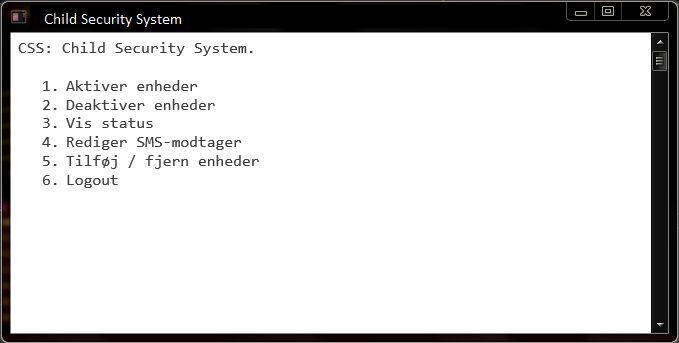
\includegraphics[width=0.75\textwidth]{billeder/cmdprompt/CSS_menu}}
\caption{CSS Menu}
%\label{lab:CSS Menu}
\end{figure}

\begin{figure}[h] \centering
{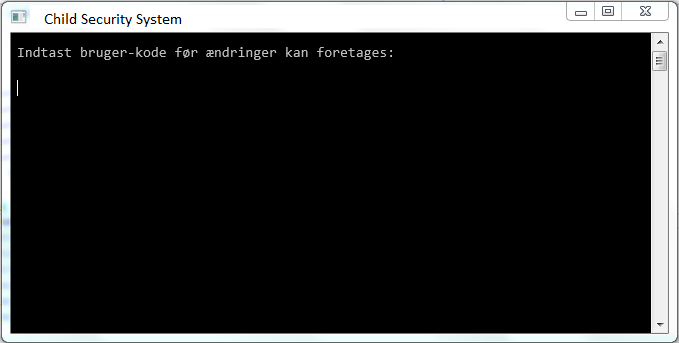
\includegraphics[width=0.75\textwidth]{billeder/cmdprompt/CSS_login}}
\caption{CSS Login}
%\label{fig:CSS Login}
\end{figure}

\begin{figure}[h] \centering
{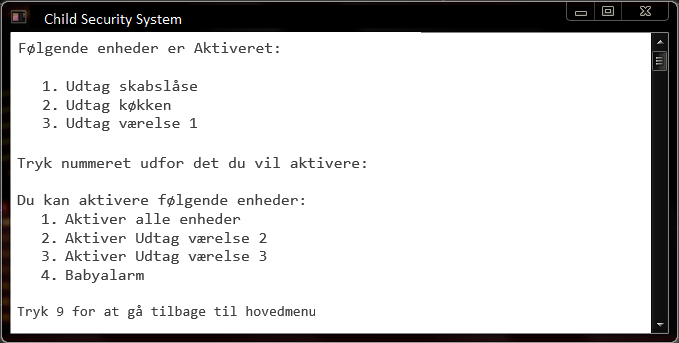
\includegraphics[width=0.75\textwidth]{billeder/cmdprompt/CSS_aktiver}}
\caption{CSS Aktiver}
%\label{fig:CSS Aktiver}
\end{figure}

\begin{figure}[h] \centering
{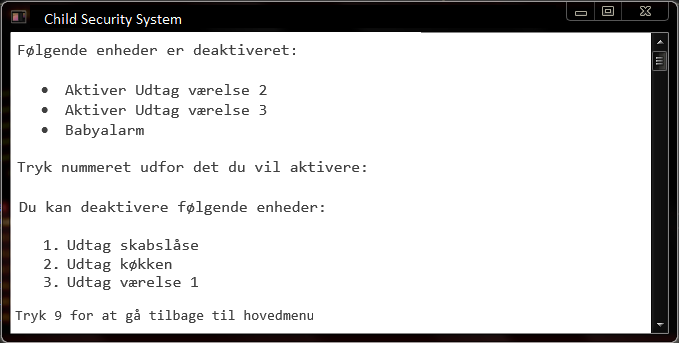
\includegraphics[width=0.75\textwidth]{billeder/cmdprompt/CSS_deaktiver}}
\caption{CSS Deaktvier}
%\label{fig:CSS Deaktvier}
\end{figure}

\begin{figure}[h] \centering
{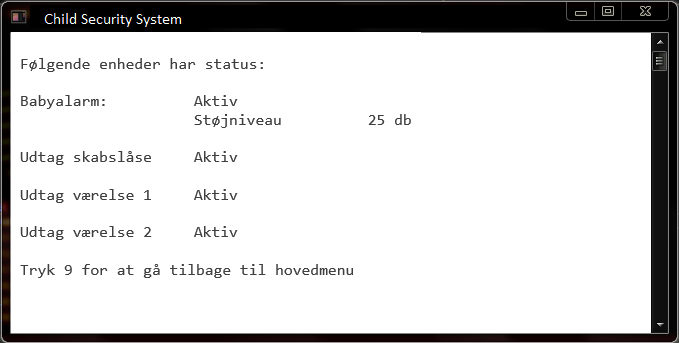
\includegraphics[width=0.75\textwidth]{billeder/cmdprompt/CSS_vis_status}}
\caption{CSS Vis Status}
%\label{fig:CSS Vis Status}
\end{figure}

\begin{figure}[h] \centering
{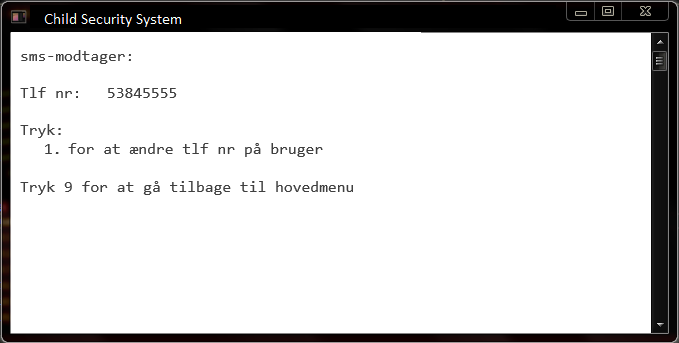
\includegraphics[width=0.75\textwidth]{billeder/cmdprompt/CSS_advisering}}
\caption{CSS Advisering}
%\label{fig:CSS Advisering}
\end{figure}



